\section{Further Generalisation Experiment Details}\label{app:further_generalise}

\begin{figure*}[htbp]
    \centering
    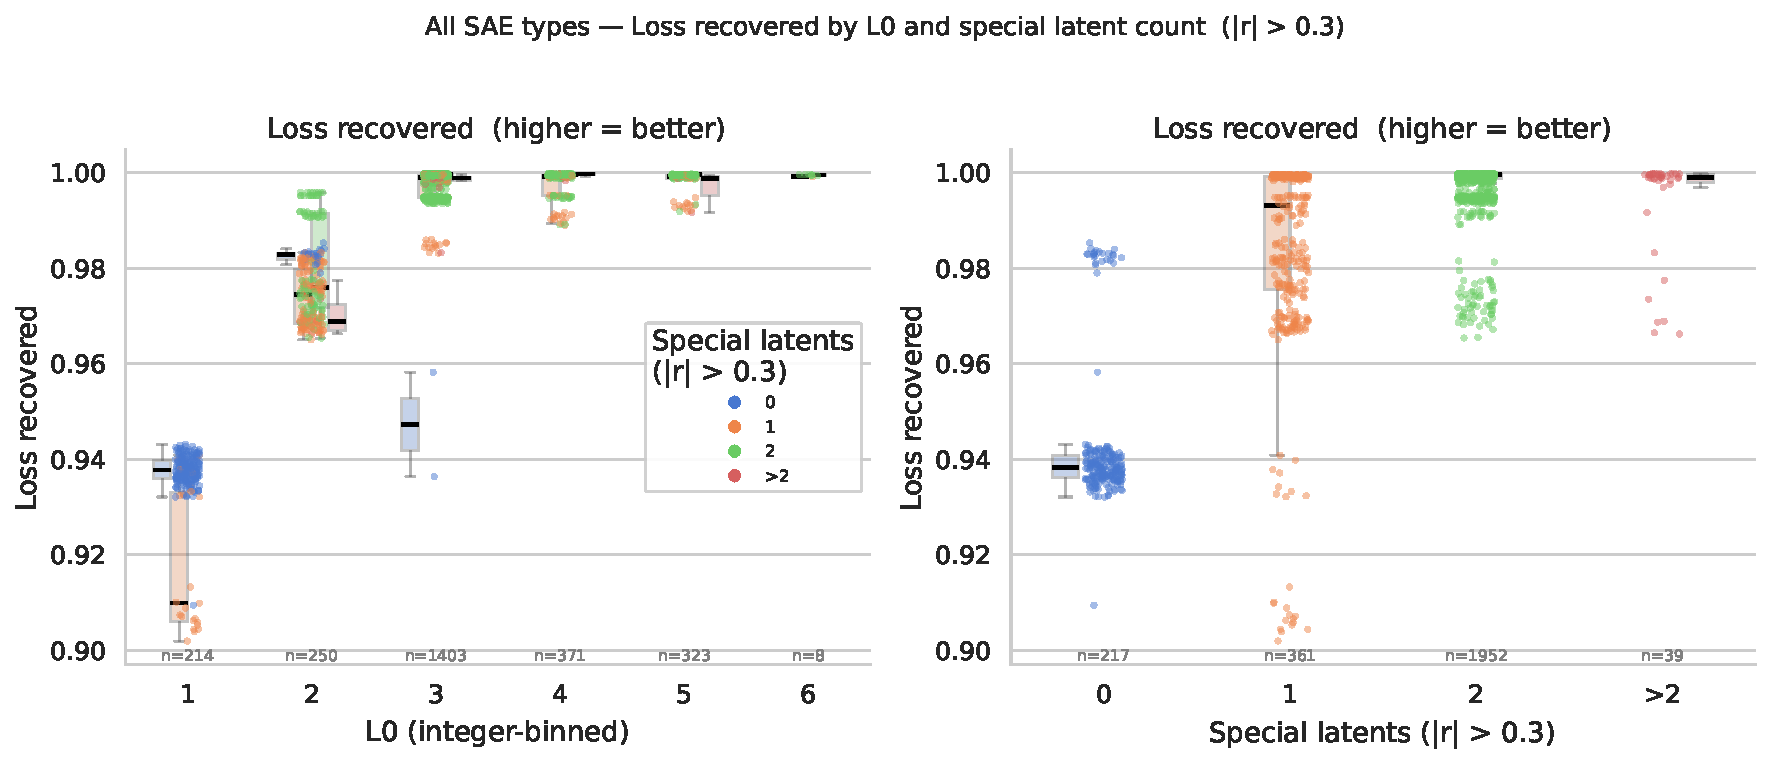
\includegraphics[width=\linewidth]{figures/special_latents_vs_performance.pdf}
    \caption{These strip plots show how the number of special latents (identified by the latent's activation's correlation with $\Delta \alpha$ using threshold $|r| > 0.3$, % TODO note that these plots actually use 0.5 so i'm lying here (can fix for actual paper but okay for now)
    as in Section \ref{ss:sae_feat_analysis}) differs across SAEs with different performance.
    It shows that SAEs with strong performance, measured by explained variance and patched cross-entropy loss, tend to have 2 special latents (spearman $r=-0.460$ for patched cross-entropy loss and $r=0.506$ for explained variance).}
    \label{fig:special_latents_vs_performance}
\end{figure*}

% TODO


% TODO could add table showing % of saes with 2 special have 1 d1 favouring the other d2 favouring (+ average corrs?). and saes with 1 special % d1 favouring and % d2 favouring + avg corrs

To test whether special latents can be steered to swap outputs in other SAEs, we provide the following pipeline that works given any SAE, which is available in our public codebase:
\begin{enumerate}
    \item Store the SAE activations for all input bigrams by running a single 
    forward pass as in Figure \ref{fig:rq2_pipeline} over the full dataset and recording each SAE latent's activation 
    magnitude.
    \item Identify special latents using $\Delta \alpha$ correlation $|r|>0.3$ as a heuristic, 
    as described previously.
    \item For each identified special latent, run a batched steering grid search 
    over all input bigrams. For each bigram and each scale factor 
    $p \in [0,10]$ with step size 0.05 (201 values), record the logits at 
    output positions $o_1$ and $o_2$ under the steered reconstruction 
    $\hat{\boldsymbol{r}}_{s}^{L_1}$. Bigrams for which the latent does not 
    activate ($m = 0$) are skipped immediately since scaling has no effect.
    
    \item Find crossover scales for each bigram:
    \begin{itemize}
        \item For $o_1$: since $o_1$ logits are empirically linear in $p$, fit 
        lines to $\ell_{d_1}(p)$ and $\ell_{d_2}(p)$ and compute the analytical 
        intersection. Inputs for which either logit series fails an $R^2 \geq 0.999$ 
        linearity check, or for which the intersection falls on a negative scale, are flagged and excluded.
        \item For $o_2$: detect sign changes in $\ell_{d_1}(p) - \ell_{d_2}(p)$ 
        on the coarse $[0, 10]$ grid, then refine each crossing to three decimal places using 
        bisection search. All bisection tasks across the batch are executed in parallel to 
        avoid sequential per-input forward passes.
    \end{itemize}
    
    \item Determine a valid swap zone $[p_{\mathrm{lo}}, p_{\mathrm{hi}}]$ per 
    bigram by intersecting the $o_1$ and $o_2$ crossover constraints with the 
    scale ranges over which $\mathrm{argmax}(o_1) = d_2$ and 
    $\mathrm{argmax}(o_2) = d_1$ hold simultaneously. If no contiguous window 
    satisfying both conditions exists, the bigram is recorded as a failure with a 
    specific reason (see Section \ref{ss:steering_exp}).
    
    \item Verify each swap zone by running the model at the midpoint 
    $p^* = (p_{\mathrm{lo}} + p_{\mathrm{hi}})/2$ and confirming that the model 
    output is $(d_2, d_1)$.
    
    \item Report the fraction of bigrams for which a valid swap zone was found and 
    the swap verified, along with a breakdown of failure reasons for the remainder.
\end{enumerate}
Steps 3-5 of the pipeline are very computationally expensive, so we test generalisation using a varied sample of six high performing SAEs (Table \ref{tab:cherry-picked-saes}) rather than running the pipeline on all trained SAEs (as in Figure \ref{fig:special_latents_vs_performance}).
The results are shown in Table \ref{tab:steering_generalisation}.

In future work, this study should be extended to further configurations for robust statistical significance.